\documentclass[17pt]{memoir}
\usepackage[letterpaper,landscape,left=1.5cm,right=1.5cm,top=1.5cm,bottom=1.5cm]{geometry}
\usepackage[spanish]{babel}
\usepackage[utf8]{inputenc}
\usepackage[T1]{fontenc}
%configuración de fuentes, colores y gráficos
\usepackage{pslatex}
\usepackage[pdftex]{graphicx}
\usepackage[dvipsnames]{color}
\definecolor{unablue}{rgb}{0,0,0.2}
\definecolor{light-gray}{gray}{0.85}
\definecolor{dark-gray}{gray}{0.20}
\definecolor{shadecolor}{gray}{0.85}
\definecolor{medium-gray}{gray}{0.50}
\usepackage{tikz}

\usepackage[code=2/5-Datalogic,X=.6mm,ratio=3,H=0.8cm]{makebarcode}

\renewcommand{\sfdefault}{phv}
\renewcommand*{\familydefault}{\sfdefault}

\hyphenpenalty 100000

%variables
\newcommand{\centrolocal}{ANZOATEGUI}
\newcommand{\clua}{0201}
\newcommand{\aspirante}{Romero Palma, José Loreto}
\newcommand{\cedula}{13257153}
\newcommand{\lapsoguion}{2013-2}
\newcommand{\lapso}{20132}
\newcommand{\ciudad}{El Tigre}
\newcommand{\dia}{18}
\newcommand{\mes}{octubre}
\newcommand{\anho}{2013}
\newcommand{\orientador}{Lcda. Nancy Bello}
\newcommand{\tituloorientador}{Orientadora}



\begin{document}
	\pagestyle{empty} 
	\begin{center}
		\setlength{\unitlength}{1cm}
		\begin{picture}(24.5,18.3)
			\put(0,0){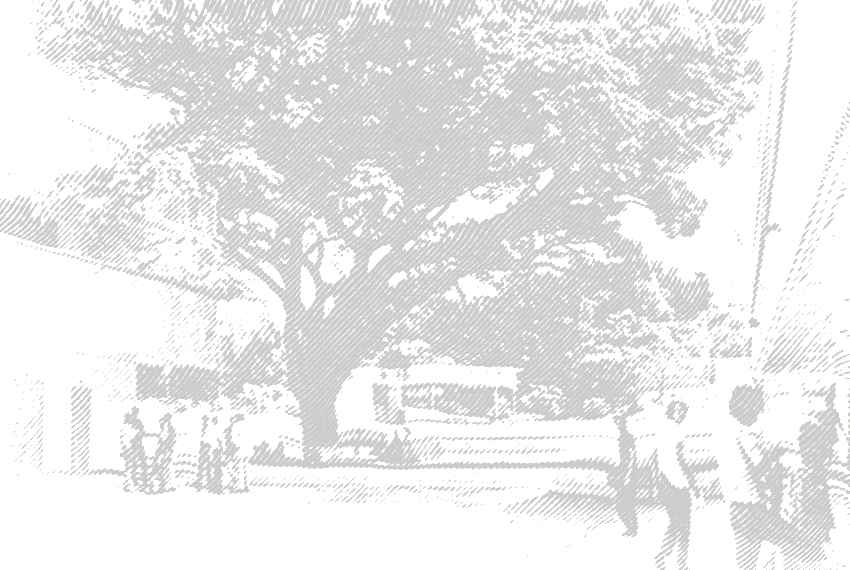
\includegraphics[width=\textwidth,height=\textheight]{saman.jpg}}
			\put(2.2,17.7){
				\begin{tabular}{lcr}
					\barcode{\clua}	& \barcode{\cedula} & \barcode{\lapso}\\[-1.2ex]
					\parbox{4ex}{\centering \tiny \clua} & \parbox{39.5ex}{\centering \tiny \hspace{2ex} \cedula} &
					\parbox{5ex}{\centering \tiny \hspace{2ex} \lapso}
				\end{tabular}
			}
			\put(5.8,14.7){\parbox{56ex}{\centering 
				\fontsize{32}{40}\selectfont \textsc{ \textcolor{unablue}{Universidad Nacional Abierta}} \\[-1ex]
				\fontsize{26}{40}\selectfont \textsc{ \textcolor{unablue}{Vicerectorado Académico}} \\[-1.4ex]
				\fontsize{20}{40}\selectfont \textsc{ \textcolor{unablue}{CL \centrolocal}} }
			}
			%el logotipo
			\put(2.6,13.6){
				\begin{tikzpicture}[scale=2.6]
					\filldraw[fill=blue!30!black, draw=black] (0,1) -- (0,0.77) -- (0.3,0.46) -- (0.3,0.69) -- cycle;
					\filldraw[fill=blue!30!black, draw=black] (0,0.54) -- (0,0.31) -- (0.26,0.04) -- (0.29,0.02) -- (0.32,0.01) -- (0.35,0.02) -- (0.38,0.04) -- (0.39,0.06) -- (0.4,0.1) -- (0.4,0.69) -- (0.43,0.73) -- (0.45,0.74) -- (0.48,0.73) -- (0.72,0.46) -- (0.72,0.70) -- (0.50,0.95) -- (0.47,0.97) -- (0.43,0.98) -- (0.39,0.97) -- (0.36,0.95) --(0.35,0.93) -- (0.34,0.89) -- (0.34,0.28) -- (0.31,0.27) -- (0.28,0.28) -- cycle;
					\filldraw[fill=blue!30!black, draw=black] (0.44,0.54) -- (0.44,0.31) -- (0.70,0.04) -- (0.73,0.02) -- (0.76,0.01) -- (0.79,0.02) -- (0.82,0.04) -- (0.83,0.06) -- (0.84,0.1) -- (0.84,0.69) -- (0.87,0.73) -- (0.89,0.74) -- (0.92,0.73) -- (1.16,0.46) -- (1.16,0.70) -- (0.94,0.95) -- (0.91,0.97) -- (0.87,0.98) -- (0.83,0.97) -- (0.80,0.95) --(0.79,0.93) -- (0.78,0.89) -- (0.78,0.28) -- (0.75,0.27) -- (0.72,0.28) -- cycle;
					\filldraw[fill=blue!30!black, draw=black] (0.88,0.54) -- (0.88,0.31) -- (1.16,0.01) -- (1.16,0.24) -- cycle;
				\end{tikzpicture}
			}
			\put(2.3,11.4){\parbox{66ex}{ \centering
				\fontsize{28}{40}\selectfont \textsc{ \textcolor{black}{CERTIFICADO DE APROBACION}} }
			}
			%cuerpo principal
			\put(2.7,8.6){\parbox{66ex}{
			  \fontsize{20}{24}\selectfont Por medio del presente se hace constar que el(la) aspirante \textbf{\aspirante}, titular de la Cédula de Identidad \textbf{\cedula}, aprobó satisfactoriamente el \textbf{Curso Introductorio} en el lapso \lapsoguion. \par}
			}
			%se expide en
			\put(2.7,5.8){\parbox{66ex}{
			  \fontsize{20}{24}\selectfont Constancia que se expide en \ciudad {} a los \dia {} del mes de \mes {} del año \anho. \par}
			}
			%firma
			\put(2.7,0.5){\parbox{66ex}{\centering
				\fontsize{20}{24}
				\rule{20ex}{0.5pt} \\
				\orientador \\
				\tituloorientador \par}
			}
		\end{picture}
	\end{center}
\end{document}
